\documentclass[12pt]{article}
\usepackage{listings}
\usepackage{caption}
\DeclareCaptionFont{white}{\color{white}}
\DeclareCaptionFormat{listing}{%
	\parbox{\textwidth}{\colorbox{gray}{\parbox{\textwidth}{#1#2#3}}\vskip-4pt}}
\captionsetup[lstlisting]{format=listing,labelfont=white,textfont=white}
\lstset{frame=lrb,xleftmargin=\fboxsep,xrightmargin=-\fboxsep}

\usepackage{color}
\usepackage{xcolor}

\usepackage{xparse}

\usepackage{graphicx}
\graphicspath{ {.} }

\NewDocumentCommand{\codeword}{v}{%
	\texttt{\textcolor{blue}{#1}}%
}

\definecolor{dkgreen}{rgb}{0,0.6,0}
\definecolor{gray}{rgb}{0.5,0.5,0.5}
\definecolor{mauve}{rgb}{0.58,0,0.82}

\lstset{frame=tb,
	language=Java,
	aboveskip=3mm,
	belowskip=3mm,
	showstringspaces=false,
	columns=flexible,
	basicstyle={\small\ttfamily},
	numbers=none,
	numberstyle=\tiny\color{gray},
	keywordstyle=\color{blue},
	commentstyle=\color{dkgreen},
	stringstyle=\color{mauve},
	breaklines=true,
	breakatwhitespace=true,
	tabsize=3
}

\newenvironment{solution}[1][]{
	\vspace{10px}\noindent\emph{Solution #1}
}{
	\vspace{10px}
}

\begin{document}

	\section*{Problem 19}
	The \codeword{evaluate()} method works out how accurately the tagger performs on this text. For example, if the supplied tagged text was \codeword{[('the', 'DT'), ('dog', 'NN')]} and the tagger produced the output \codeword{[('the', 'NN'), ('dog', 'NN')]}, then the score would be 0.5. Let's try to figure out how the evaluation method works:
	\begin{enumerate}
		\item A tagger \codeword{t} takes a list of words as input, and produces a list of tagged words as output. However, \codeword{t.evaluate()} is given correctly tagged text as its only parameter. What must it do with this input before performing the tagging?
		
		Strip the tags from the gold standard text.
		
		\item Once the tagger has created newly tagged text, how might the \codeword{evaluate()} method go about comparing it with the original tagged text and computing the accuracy score?
		
		For each work in the tagged output, it would compare whether or not the tag of that word matches the tag of the same word from the gold standard input.
		
		\item Now examine the source code to see how the method is implemented. Inspect \codeword{nltk.tag.api.__file__} to discover the location of the source code, and open this file using an editor.\\
		
		Source Code for \codeword{evaluate()}:
		\begin{lstlisting}
		def evaluate(self, gold):
			"""
			Score the accuracy of the tagger against the gold standard.
			Strip the tags from the gold standard text, retag it using
			the tagger, then compute the accuracy score.
			
			:type gold: list(list(tuple(str, str)))
			:param gold: The list of tagged sentences to score the tagger on.
			:rtype: float
			"""
			
			tagged_sents = self.tag_sents(untag(sent) for sent in gold)
			gold_tokens = list(chain(*gold))
			test_tokens = list(chain(*tagged_sents))
			return accuracy(gold_tokens, test_tokens)
		\end{lstlisting}
	\end{enumerate}
	
	\section*{Problem 20}
	Write code to search the Brown Corpus for particular words and phrases according to tags, to answer the following questions:
	\begin{enumerate}
		\item Produce an alphabetically sorted list of the distinct words tagged as MD.
		
		Code:\\
		\begin{lstlisting}
		def sorted_tags():
			'''
			Produce an alphabetically sorted list of the distinct words tagged as MD. 
			'''
			tagged_words = nltk.corpus.brown.tagged_words()
			words_of_interest = []
			for tag_pair in tagged_words:
			if tag_pair[1] == 'MD':
			words_of_interest.append(tag_pair[0].lower())
			distinct_words_of_interest = list(set(words_of_interest))
			distinct_sorted_words_of_interest = sorted(distinct_words_of_interest, key=str.lower)
			
			print("Distinct words tagged as MD: %s" % distinct_sorted_words_of_interest)
			print("Number of distinct_words_of_interest: %s" % len(distinct_sorted_words_of_interest))
		\end{lstlisting}
		
		Output:\\
		\begin{lstlisting}
		$ python3 expanded_tagger.py
		Distinct words tagged as MD: ["c'n", 'can', 'colde', 'could', 'dare', 'kin', 'maht', 'mai', 'may', 'maye', 'mayst', 'might', 'must', 'need', 'ought', 'shall', 'should', 'shuld', 'shulde', 'wil', 'will', 'wilt', 'wod', 'wold', 'wolde', 'would']
		Number of distinct_words_of_interest: 26
		\end{lstlisting}
		
		\item Identify words that can be plural nouns or third person singular verbs (e.g. deals, flies).\\
		
		Code:
		\begin{lstlisting}
		def multi_tags():
			brown_tagged = brown.tagged_words()
			data = nltk.ConditionalFreqDist((word.lower(), tag) for (word, tag) in brown_tagged)
			words_of_interest = []
			for word in sorted(data.conditions()):
			if len(data[word]) > 2:
				tags = [tag for (tag, _) in data[word].most_common()]
				if ('VBZ' in tags and 'NNS' in tags):
					words_of_interest.append(word)
			print("Words categorized as both VBZ and NNS: ")
			print(words_of_interest)
		\end{lstlisting}
		
		Output:
		\begin{lstlisting}
		$ python3 expanded_tagger.py
		Words categorized as both VBZ and NNS:
		['accounts', 'acts', 'addresses', 'aids', 'appeals', 'associates', 'attacks', 'attempts', 'attributes', 'backs', 'bangs', 'banks', 'bars', 'bellows', 'benefits', 'boards', 'bridges', 'bugs', 'burns', 'calls', 'cares', 'causes', 'centers', 'champions', 'changes', 'charges', 'checks', 'claims', 'clouds', 'colors', 'comments', 'contacts', 'contracts', 'controls', 'costs', 'courts', 'dances', 'designs', 'dies', 'dishes', 'dogs', 'doubles', 'dreams', 'drifts', 'drinks', 'exercises', 'exhibits', 'faces', 'factors', 'falls', 'fashions', 'fears', 'features', 'feeds', 'fields', 'figures', 'flies', 'forces', 'functions', 'gains', 'guides', 'harbors', 'helps', 'hits', 'holds', 'honors', 'hopes', 'influences', 'issues', 'lands', 'levels', 'limits', 'lines', 'lists', 'lives', 'marches', 'markets', 'means', 'meets', 'misses', 'moves', 'needs', 'notes', 'objects', 'offers', 'orders', 'pictures', 'places', 'plans', 'powers', 'practices', 'projects', 'purchases', 'questions', 'rates', 'reasons', 'rebels', 'records', 'regrets', 'remains', 'remarks', 'replies', 'reports', 'results', 'returns', 'rises', 'rolls', 'rules', 'sanctions', 'services', 'sets', 'shares', 'shows', 'snows', 'speeds', 'sports', 'springs', 'stakes', 'stands', 'states', 'stems', 'steps', 'stops', 'studies', 'subjects', 'supplies', 'supports', 'switches', 'tastes', 'tests', 'times', 'tops', 'toys', 'transfers', 'travels', 'trusts', 'turns', 'uses', 'values', 'views', 'visits', 'winds', 'works']
		\end{lstlisting}
		
		\item Identify three-word prepositional phrases of the form IN + DET + NN (eg. in the lab).
		
		Code:
		\begin{lstlisting}
		def find_phrase():
			for tagged_sent in brown.tagged_sents():
				for (w1,t1), (w2,t2), (w3,t3) in nltk.trigrams(tagged_sent):
					if (t1=='IN' and t2 == 'AT' and t3=='NN'):
						print(w1, w2, w3)
		\end{lstlisting}
		
		Output:
		\begin{lstlisting}
		$python find_phrase.py
		[for the moment
		from the curio
		by a hammer
		in the subcontinent
		by a fish
		After a while
		by the process
		from the idol
		without the threat
		to a television
		to the top
		in an elevator
		to the dozen
		of a nemesis
		on the street
		of the hex
		into a seat
		across the aisle
		...]
		\end{lstlisting}
		
		\item What is the ratio of masculine to feminine pronouns?
		
		Output:
		\begin{lstlisting}
		$ python3 expanded_tagger.py
		Masculine pronouns: 12816
		Feminine pronouns: 4108
		Ratio: 3.1197663096397275
		\end{lstlisting}
		
		Code:
		\begin{lstlisting}
		def gendered_tags():
			tagged_words = nltk.corpus.brown.tagged_words(tagset='universal')
			masculine_pronouns = ['his', 'hisself',  'him','hymselfe', 'he', 'himself',"'im",'himselfe', 'hym']
			feminine_pronouns = ['herself', 'her','hers','she',]
			
			masculine_instances = 0
			feminine_instances = 0
			
			for tag_pair in tagged_words:
				if tag_pair[1] == 'PRON':
					if tag_pair[0].lower() in masculine_pronouns:
						masculine_instances += 1
					if tag_pair[0].lower() in feminine_pronouns:
						feminine_instances += 1
			
			print("Masculine pronouns: %s" % masculine_instances)
			print("Feminine pronouns: %s" % feminine_instances)
			print("Ratio: %s" % (masculine_instances / feminine_instances))
		\end{lstlisting}
		
	\end{enumerate}
	
	
	\section*{Problem 26}
	 \codeword{4.1} plotted a curve showing change in the performance of a lookup tagger as the model size was increased. Plot the performance curve for a unigram tagger, as the amount of training data is varied.
	 
	 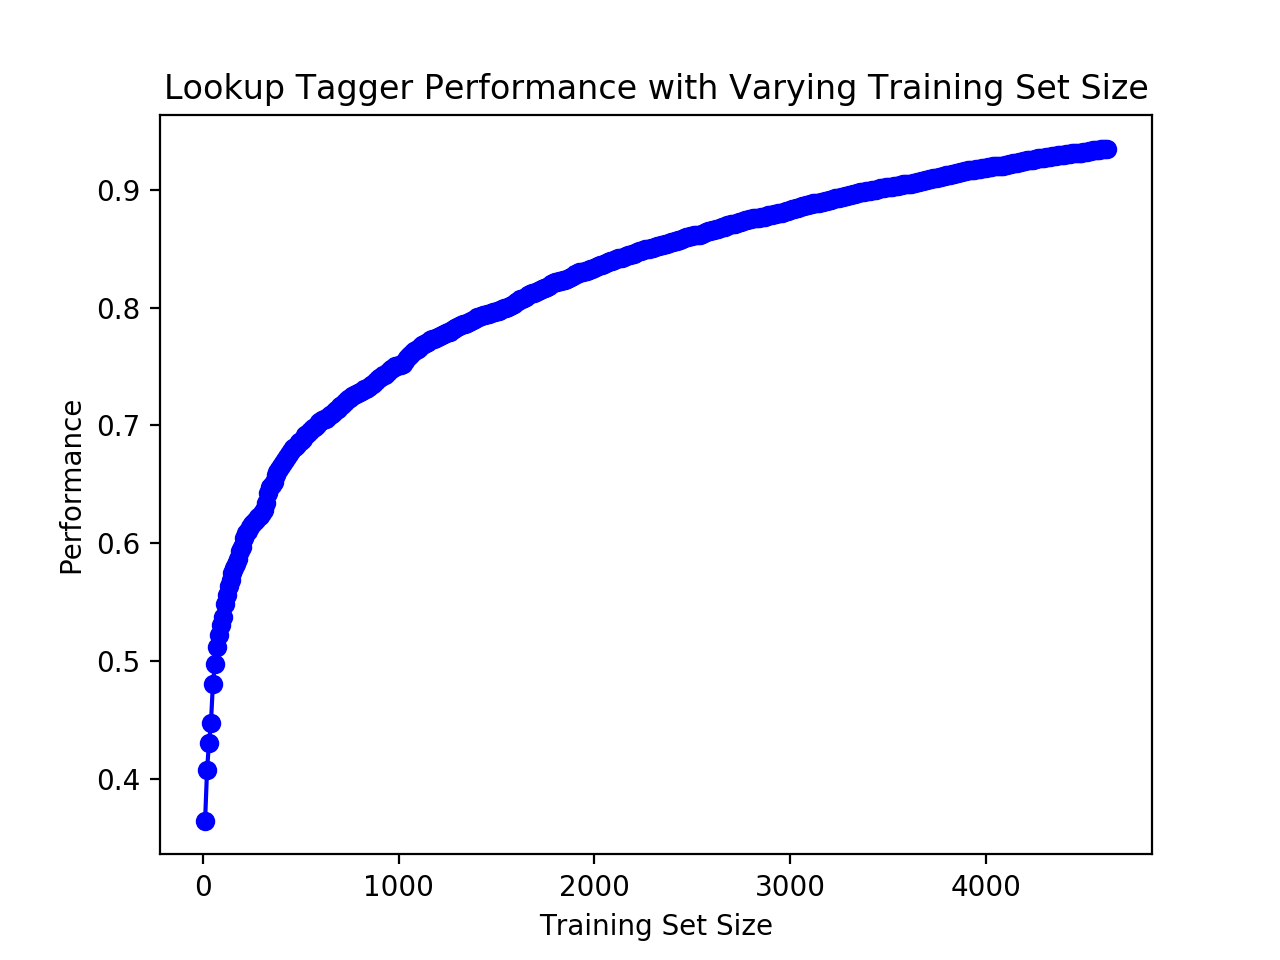
\includegraphics[scale=1.0]{Figure_1.png}.
	 
	 Code:
	 \begin{lstlisting}
	 def unigram_performance(cfd, set_size):
		 brown_tagged_sents = brown.tagged_sents(categories='news')
		 unigram_tagger = nltk.UnigramTagger(brown_tagged_sents[:set_size])
		 return unigram_tagger.evaluate(brown.tagged_sents(categories='news'))
	 
	 def display():
		 cfd = nltk.ConditionalFreqDist(brown.tagged_words(categories='news'))
		 set_sizes = list(range(10, len(brown.sents(categories='news')), 10))
		 perfs = [unigram_performance(cfd, size) for size in set_sizes]
		 pylab.plot(set_sizes, perfs, '-bo')
		 
		 pylab.title('Lookup Tagger Performance with Varying Training Set Size')
		 pylab.xlabel('Training Set Size')
		 pylab.ylabel('Performance')
		 pylab.show()
	 
	 display()
	 \end{lstlisting}
	
\end{document}
